\documentclass[journal]{IEEEtran}

% Common packages (mirror template/report/report.tex)
\usepackage{graphicx}
\usepackage{amsmath}
\usepackage{amssymb}
\usepackage{hyperref}
\usepackage{float}
\usepackage{subcaption}
\usepackage{booktabs}
\usepackage{pgfplotstable}
\usepackage{siunitx}
\usepackage{qrcode}
\usepackage{placeins}

\pgfplotsset{compat=1.18}

\pgfplotstableset{
    col sep=comma,
    every head row/.style={before row=\toprule, after row=\midrule},
    every last row/.style={after row=\bottomrule},
}

\begin{document}

% ---------- TITLE & AUTHOR ----------
\title{Heat Insulation and Conduction}
\author{Ibrahim H.I. ABUSHWISH \\
Istanbul University, Department of Physics \\
Instructor: \\
Experiment Date: 27.04.2026, Report Submission Date: \\
Course \& Section Number: PHYS3604}

\markboth{Physics Laboratory Reports, <Month Year>}{ }

\maketitle

% ---------- ABSTRACT ----------
\begin{abstract}
Heat transfer through a model-house wall was investigated for two materials (wood and normal glass) under two operating conditions: internal heating and external illumination. Inner/outer air temperatures and inner/outer wall-surface temperatures were measured and used to determine the heat flux $q=P/A$, the overall heat-transfer coefficient $k$, and the thermal conductivity $\lambda$. In addition, selected temperature series were approximated by linear models to quantify the observed time dependence. Using the measured steady-state temperature differences and the known wall thickness, the mean conductivities were found to be $\lambda_{\mathrm{wood}}=\SI{0.128}{\watt\per\meter\kelvin}$ and $\lambda_{\mathrm{glass}}=\SI{0.956}{\watt\per\meter\kelvin}$; wood therefore exhibited substantially better insulating performance than normal glass.
\end{abstract}

% ---------- INTRODUCTION ----------
\section{Introduction}
Heat losses through building envelopes are governed primarily by conduction through solid layers together with convective heat exchange at the inner and outer surfaces. In the present experiment, a model house with interchangeable wall panels was used to compare the thermal insulation properties of wood and normal glass. Inner/outer air temperatures and wall-surface temperatures were recorded during a heating phase and an illumination phase. From these measurements, the heat flux, the overall heat-transfer coefficient, and the thermal conductivity were determined, and the time evolution of selected temperatures was summarized by linear regression.

% ---------- THEORY ----------
\section{Theory}

For a plane wall at steady state, the heat flux at the inside and outside surfaces is modeled by convection:
\begin{equation}
\frac{P}{A} = \alpha_i\,\left(\theta_{\mathrm{Li}}-\theta_{\mathrm{wi}}\right)
\label{eq:q_in}
\end{equation}
\begin{equation}
\frac{P}{A} = \alpha_o\,\left(\theta_{\mathrm{wo}}-\theta_{\mathrm{Lo}}\right)
\label{eq:q_out}
\end{equation}
where $\alpha_i$ and $\alpha_o$ are the inner and outer heat-transfer coefficients, $\theta_{\mathrm{Li}}$ and $\theta_{\mathrm{Lo}}$ are the inner and outer air temperatures, and $\theta_{\mathrm{wi}}$ and $\theta_{\mathrm{wo}}$ are the inner and outer wall-surface temperatures.

The overall heat transition coefficient $k$ relates the heat flow to the air-temperature difference:
\begin{equation}
P = k\,A\,\left(\theta_{\mathrm{Li}}-\theta_{\mathrm{Lo}}\right)
\label{eq:P_overall}
\end{equation}
Combining with the heat flux gives
\begin{equation}
k = \frac{(P/A)}{\left(\theta_{\mathrm{Li}}-\theta_{\mathrm{Lo}}\right)}
\label{eq:k_def}
\end{equation}

For a homogeneous layer of thickness $d$, the conductivity can be obtained from the wall temperature drop:
\begin{equation}
\lambda = \left(\frac{P}{A}\right)\,\frac{d}{\left(\theta_{\mathrm{wi}}-\theta_{\mathrm{wo}}\right)}
\label{eq:lambda_def}
\end{equation}
The series-resistance form used to interpret $k$ is
\begin{equation}
\frac{1}{k} = \frac{1}{\alpha_i} + \frac{d}{\lambda} + \frac{1}{\alpha_o}
\label{eq:series_resistance}
\end{equation}

% ---------- EXPERIMENTAL SETUP ----------
\section{Experimental Setup}
The setup consisted of a thermally insulated model house with openings for temperature probes, four NiCr--Ni thermocouples, and a \SI{120}{\watt} incandescent lamp with reflector used as a controllable heat source. Replaceable wall panels made of wood and normal glass were mounted with thickness $d=\SI{1.00}{\centi\meter}$.

% ---------- PROCEDURE ----------
\section{Experimental Procedure}
Two phases were performed.

\textbf{Heating phase:} The interior was heated until the air temperature reached approximately \SIrange{50}{60}{\degreeCelsius}. Inner/outer air and surface temperatures were then recorded at \SI{3}{\minute} intervals for \SI{15}{\minute}.

\textbf{Illumination phase:} The outer wall was illuminated by the lamp placed at approximately \SI{15}{\centi\meter}. Temperatures were recorded at \SI{1}{\minute} intervals for \SI{5}{\minute} for each material.

For the analysis, the natural-convection coefficients were taken as $\alpha_i=\alpha_o=\SI{8.10}{\watt\per\meter\squared\kelvin}$.

% ---------- DATA ANALYSIS ----------
\section{Data Analysis}
The heat flux through the wall was obtained from the measured outside-surface and outside-air temperatures using Eq.~\eqref{eq:q_out} together with the assumed convective coefficient. The overall heat-transfer coefficient was then calculated from Eq.~\eqref{eq:k_def} using the inner--outer air temperature difference. Finally, the thermal conductivity of each panel was determined from Eq.~\eqref{eq:lambda_def} using the measured wall temperature drop and the known thickness.

To characterize the temperature evolution during each phase, selected temperature series were fitted with a linear model $y=mt+b$. The fitted slope and intercept provide a compact measure of heating/cooling rate over the measurement interval, while the coefficient of determination $R^2$ was used to indicate the quality of the linear approximation.

% ---------- RESULTS ----------
\section{Results}

\subsection{Data Tables}

\begin{table*}[t]
    \centering
    \caption{Heating phase measurements (Table 2). Values are given to 3 significant figures.}
    \label{tab:heating_measurements}
    \pgfplotstabletypeset[
        string type,
        columns/time_min/.style={column name={Time (min)}},
        columns/air_in_C/.style={column name={$\theta_{\mathrm{Li}}$ (\si{\degreeCelsius})}},
        columns/air_out_C/.style={column name={$\theta_{\mathrm{Lo}}$ (\si{\degreeCelsius})}},
        columns/wood_in_C/.style={column name={Wood $\theta_{\mathrm{wi}}$ (\si{\degreeCelsius})}},
        columns/wood_out_C/.style={column name={Wood $\theta_{\mathrm{wo}}$ (\si{\degreeCelsius})}},
        columns/glass_in_C/.style={column name={Glass $\theta_{\mathrm{wi}}$ (\si{\degreeCelsius})}},
        columns/glass_out_C/.style={column name={Glass $\theta_{\mathrm{wo}}$ (\si{\degreeCelsius})}},
    ]{tables/heating_measurements_table2.csv}
\end{table*}

\begin{table*}[t]
    \centering
    \caption{Illumination phase measurements for wood (Table 4a). Values are given to 3 significant figures.}
    \label{tab:illumination_wood_measurements}
    \pgfplotstabletypeset[
        string type,
        columns/time_min/.style={column name={Time (min)}},
        columns/air_in_C/.style={column name={$\theta_{\mathrm{Li}}$ (\si{\degreeCelsius})}},
        columns/air_out_C/.style={column name={$\theta_{\mathrm{Lo}}$ (\si{\degreeCelsius})}},
        columns/wood_in_C/.style={column name={Wood $\theta_{\mathrm{wi}}$ (\si{\degreeCelsius})}},
        columns/wood_out_C/.style={column name={Wood $\theta_{\mathrm{wo}}$ (\si{\degreeCelsius})}},
    ]{tables/illumination_w_measurements_table4.csv}
\end{table*}

\begin{table*}[t]
    \centering
    \caption{Illumination phase measurements for normal glass (Table 4b). Values are given to 3 significant figures.}
    \label{tab:illumination_glass_measurements}
    \pgfplotstabletypeset[
        string type,
        columns/time_min/.style={column name={Time (min)}},
        columns/air_in_C/.style={column name={$\theta_{\mathrm{Li}}$ (\si{\degreeCelsius})}},
        columns/air_out_C/.style={column name={$\theta_{\mathrm{Lo}}$ (\si{\degreeCelsius})}},
        columns/glass_in_C/.style={column name={Glass $\theta_{\mathrm{wi}}$ (\si{\degreeCelsius})}},
        columns/glass_out_C/.style={column name={Glass $\theta_{\mathrm{wo}}$ (\si{\degreeCelsius})}},
    ]{tables/illumination_g_measurements_table4.csv}
\end{table*}

\begin{table*}[t]
    \centering
    \caption{Derived quantities for the heating phase (Table 3). Values are given to 3 significant figures.}
    \label{tab:heating_derived}
    \pgfplotstabletypeset[
        string type,
        columns/phase/.style={column name={Phase}},
        columns/material/.style={column name={Material}},
        columns/d_cm/.style={column name={$d$ (\si{\centi\meter})}},
        columns/q_out_W_m2/.style={column name={$q=P/A$ (\si{\watt\per\meter\squared})}},
        columns/k_W_m2K/.style={column name={$k$ (\si{\watt\per\meter\squared\kelvin})}},
        columns/lambda_W_mK/.style={column name={$\lambda$ (\si{\watt\per\meter\kelvin})}},
        columns/Lambda_W_m2K/.style={column name={$\Lambda$ (\si{\watt\per\meter\squared\kelvin})}},
    ]{tables/heating_derived_table3.csv}
\end{table*}

\begin{table*}[t]
    \centering
    \caption{Derived quantities for the illumination phase (Table 5). Values are given to 3 significant figures.}
    \label{tab:illumination_derived}
    \pgfplotstabletypeset[
        string type,
        columns/phase/.style={column name={Phase}},
        columns/material/.style={column name={Material}},
        columns/d_cm/.style={column name={$d$ (\si{\centi\meter})}},
        columns/q_out_W_m2/.style={column name={$q=P/A$ (\si{\watt\per\meter\squared})}},
        columns/k_W_m2K/.style={column name={$k$ (\si{\watt\per\meter\squared\kelvin})}},
        columns/lambda_W_mK/.style={column name={$\lambda$ (\si{\watt\per\meter\kelvin})}},
        columns/Lambda_W_m2K/.style={column name={$\Lambda$ (\si{\watt\per\meter\squared\kelvin})}},
    ]{tables/illumination_derived_table5.csv}
\end{table*}

\FloatBarrier

\subsection{Graphs}

Only the regression plots are included below to summarize the dominant temperature trends observed in each phase.

\begin{figure}[H]
    \centering
    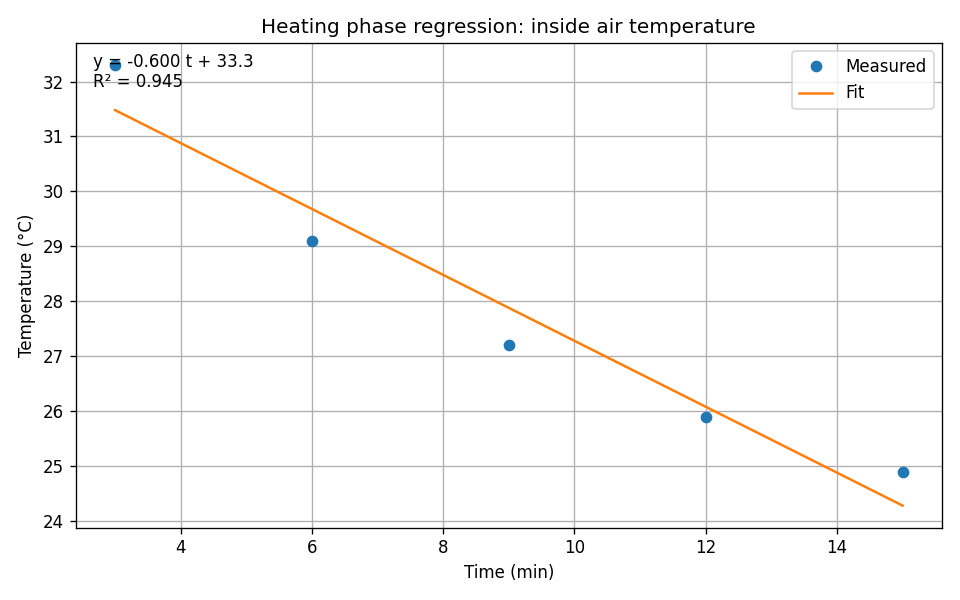
\includegraphics[width=\linewidth]{../plots/heating_air_temp_regression.png}
    \caption{Regression plot for heating phase (air): $y=-0.600t+33.3$, $R^2=0.945$ (3 significant figures).}
    \label{fig:reg_heating_air}
\end{figure}

\begin{figure}[H]
    \centering
    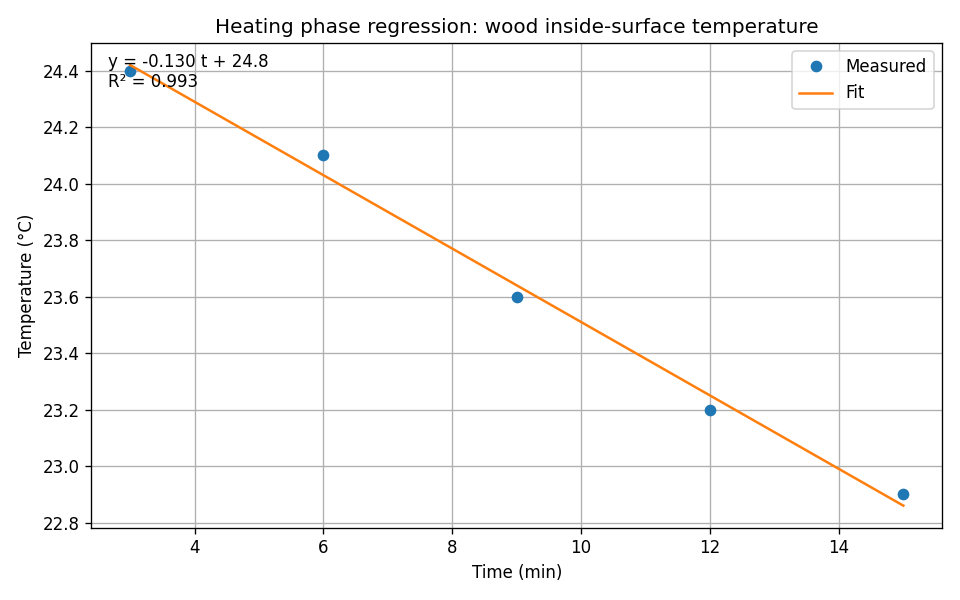
\includegraphics[width=\linewidth]{../plots/heating_w_temp_regression.png}
    \caption{Regression plot for heating phase (wood): $y=-0.130t+24.8$, $R^2=0.993$ (3 significant figures).}
    \label{fig:reg_heating_wood}
\end{figure}

\begin{figure}[H]
    \centering
    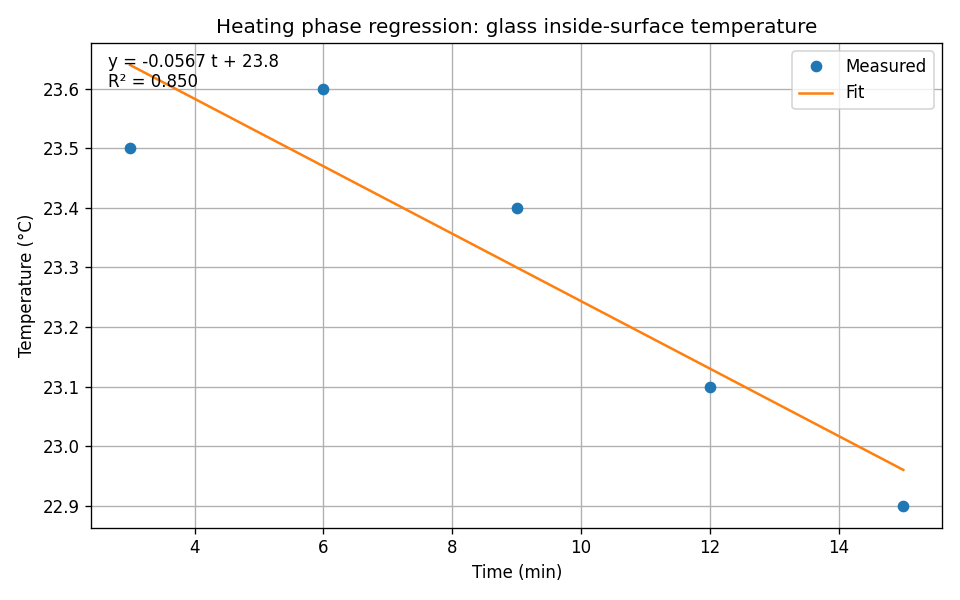
\includegraphics[width=\linewidth]{../plots/heating_g_temp_regression.png}
    \caption{Regression plot for heating phase (glass): $y=-0.0567t+23.8$, $R^2=0.850$ (3 significant figures).}
    \label{fig:reg_heating_glass}
\end{figure}

\begin{figure}[H]
    \centering
    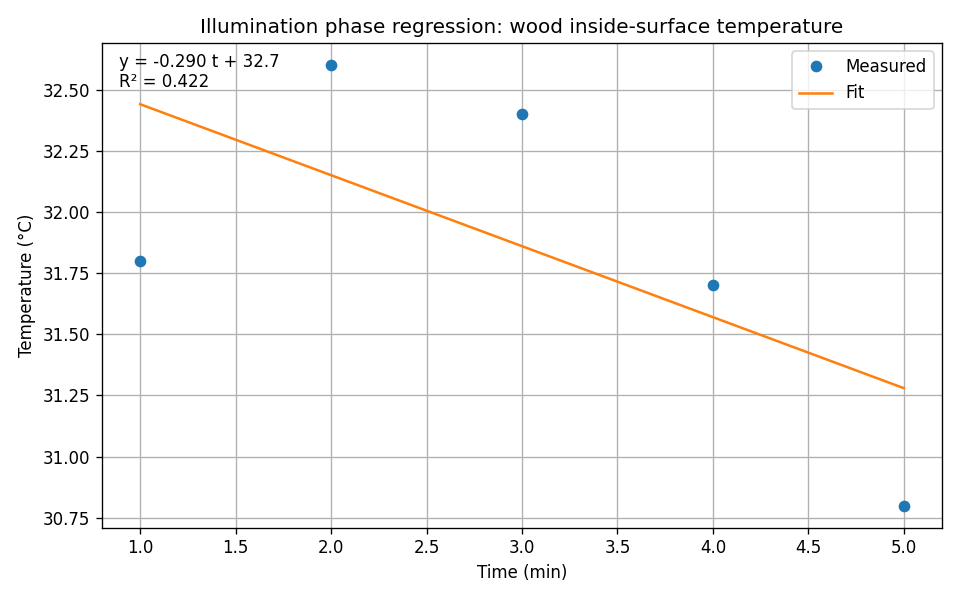
\includegraphics[width=\linewidth]{../plots/illumination_w_temp_regression.png}
    \caption{Regression plot for illumination phase (wood): $y=-0.290t+32.7$, $R^2=0.422$ (3 significant figures).}
    \label{fig:reg_illumination_wood}
\end{figure}

\begin{figure}[H]
    \centering
    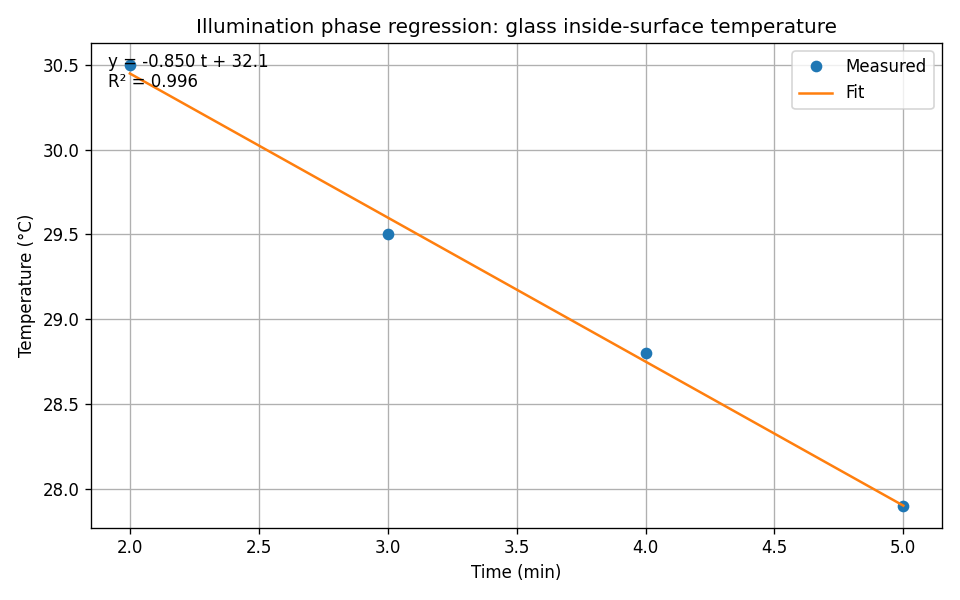
\includegraphics[width=\linewidth]{../plots/illumination_g_temp_regression.png}
    \caption{Regression plot for illumination phase (glass): $y=-0.850t+32.1$, $R^2=0.996$ (3 significant figures).}
    \label{fig:reg_illumination_glass}
\end{figure}

% ---------- DISCUSSION ----------
\section{Discussion}
The extracted conductivities show that normal glass conducts heat far more effectively than wood. Using the representative values summarized in Table~\ref{tab:heating_derived}, $\lambda_{\mathrm{glass}}=\SI{0.956}{\watt\per\meter\kelvin}$ is significantly larger than $\lambda_{\mathrm{wood}}=\SI{0.128}{\watt\per\meter\kelvin}$, which is consistent with the qualitative expectation that wood is a better thermal insulator.

The regression figures provide a quantitative summary of the observed thermal transients. During the heating measurements, the wood surface temperature was well-approximated by a linear trend over the recorded interval ($R^2=0.993$; Figure~\ref{fig:reg_heating_wood}), whereas the glass surface temperature displayed greater deviation from linearity ($R^2=0.850$; Figure~\ref{fig:reg_heating_glass}), consistent with the different thermal response of the two materials. During illumination, the glass series was almost perfectly linear ($R^2=0.996$; Figure~\ref{fig:reg_illumination_glass}), while the wood series exhibited a weaker linear correlation ($R^2=0.422$; Figure~\ref{fig:reg_illumination_wood}), indicating that additional transient effects (e.g., changing convection conditions and thermal lag) influenced the measurements.

Dominant sources of uncertainty include thermocouple placement and thermal contact, departures from the assumed constant values of $\alpha_i$ and $\alpha_o$ due to changing convection conditions, radiative exchange (particularly relevant for glass), and the limited time window for establishing strict steady state.

% ---------- CONCLUSION ----------
\section{Conclusion}

Heat transfer through wood and normal-glass wall panels was measured and analyzed using steady-state heat-transfer relations for convection at the surfaces and conduction through the wall. The mean thermal conductivity of wood was found to be $\SI{0.128}{\watt\per\meter\kelvin}$, substantially lower than that of normal glass ($\SI{0.956}{\watt\per\meter\kelvin}$), confirming wood as the better insulating material in this setup. Linear regression of selected temperature series provided concise estimates of the heating/cooling rates over the recorded intervals.

% ---------- ADDITIONAL RESOURCES ----------
\section{Additional Resources}
\newcommand{\RepoURL}{https://github.com/ibeuler/LAB-Reports}

\begin{figure}[H]
    \centering
    \begin{minipage}{0.15\textwidth}
        \centering
        \qrcode[height=1.5cm]{\RepoURL}
    \end{minipage}%
    \begin{minipage}{0.2\textwidth}
        \raggedright
        \caption{Access the repository for source files and raw data: \url{\RepoURL}.}
        \label{fig:qr_code}
    \end{minipage}
\end{figure}

\begin{thebibliography}{9}

\bibitem{labmanual}
Istanbul University, Department of Physics, \textit{Heat Insulation and Conduction} (laboratory manual).

\end{thebibliography}

\end{document}
